% =============================================================================
%  main_paper_b.tex
%  Journal Paper B — IEEE Transactions on Industrial Electronics
%
%  Title: Hilbert-Fortescue Sequence Estimation and Greedy Cascade
%         Coordination for Adaptive Overcurrent Protection of
%         Multi-Generator Busbars
%
%  Compile:
%    pdflatex main_paper_b && bibtex main_paper_b &&
%    pdflatex main_paper_b && pdflatex main_paper_b
% =============================================================================

\documentclass[journal,twoside,10pt]{IEEEtran}

% ---- Essential packages -----------------------------------------------------
\usepackage[T1]{fontenc}
\usepackage[utf8]{inputenc}
\usepackage{mathptmx}
\usepackage{microtype}

% ---- Mathematics ------------------------------------------------------------
\usepackage{amsmath,amssymb,mathtools}
\usepackage{amsthm}
\usepackage{bm}
\usepackage{siunitx}
\sisetup{detect-all,per-mode=symbol,range-phrase=\,--\,}

% ---- Figures and tables -----------------------------------------------------
\usepackage{graphicx}
\usepackage{subcaption}
\usepackage{booktabs}
\usepackage{array}
\usepackage{multirow}
\usepackage{float}

% ---- References -------------------------------------------------------------
\usepackage[colorlinks=false]{hyperref}
\usepackage{xcolor}
\bibliographystyle{IEEEtran}

% ---- Algorithm --------------------------------------------------------------
\usepackage{algorithm}
\usepackage{algpseudocode}
\renewcommand{\algorithmicrequire}{\textbf{Input:}}
\renewcommand{\algorithmicensure}{\textbf{Output:}}

% ---- Theorem environments ---------------------------------------------------
\newtheorem{theorem}{Theorem}
\newtheorem{proposition}{Proposition}
\newtheorem{remark}{Remark}

% ---- Custom macros ----------------------------------------------------------
\newcommand{\vect}[1]{\bm{#1}}
\newcommand{\mat}[1]{\mathbf{#1}}
\newcommand{\norm}[1]{\left\|#1\right\|}
\newcommand{\pu}{\,\text{pu}}
\newcommand{\mss}{\,\text{ms}}
\newcommand{\sss}{\,\text{s}}

% =============================================================================
\begin{document}
% =============================================================================

% ---- Title and authors ------------------------------------------------------
\title{Hilbert--Fortescue Sequence Estimation and\\
       Greedy Cascade Coordination for Adaptive\\
       Overcurrent Protection of Multi-Generator Busbars}

\author{Anoop~V.~Eluvathingal,~\IEEEmembership{Student Member,~IEEE,}
        and~K.~Shanti~Swarup,~\IEEEmembership{Senior Member,~IEEE}%
\thanks{Manuscript received \today.
        This work is part of the PhD research programme at the Department of
        Electrical Engineering, Indian Institute of Technology Madras,
        Chennai~600~036, India.}%
\thanks{A.~V.~Eluvathingal and K.~S.~Swarup are with the Department of
        Electrical Engineering, IIT Madras, Chennai~600~036, India
        (e-mail: ee21d017@smail.iitm.ac.in; swarup@ee.iitm.ac.in).}}

\markboth{IEEE Transactions on Industrial Electronics,~Vol.~XX,
          No.~XX, XXXX~2026}%
{Eluvathingal \& Swarup: Sequence Estimation and Cascade Coordination}

\maketitle

% =============================================================================
\begin{abstract}
Overcurrent relays protecting synchronous generator busbars use settings fixed
at commissioning that are insensitive to fault type and do not provide
coordinated selectivity across parallel generators.
This paper extends a real-time inverse parameter estimation framework
(Milestone~1, Paper~A) in two directions.
First, a Hilbert--Fortescue sequence-component estimator (M3) decomposes
three-phase fault currents into instantaneous positive-, negative-, and
zero-sequence signals and fits the Levenberg--Marquardt (LM) estimator
independently to each active sequence, enabling relay adaptation under
asymmetric fault conditions.
Second, a greedy cascade coordination algorithm (M4) enforces pickup
selectivity ($\Delta I_m \geq 0.20$\,pu) and IEC~60255 time-grading
($\Delta t_{\text{grade}} \geq 0.15$\,s) across all $N$ generator relays
in a single forward pass of exactly $N$ steps, proven by induction.
For a single-line-to-ground (SLG) fault, the sequence estimator achieves
a confidence score $\gamma = 0.914 > 0.70$, reducing pickup from
$1.20$\,pu to $1.10$\,pu ($-8.3\%$).
For a line-to-line (LL) fault, $\gamma = 0.587$ and fixed settings are
safely retained.
The cascade algorithm satisfies all coordination constraints for
$N \in \{2,3,4\}$ generators and degrades gracefully when estimation
is rejected, restoring coordination from fixed commissioning settings.
Total compute time (sequence estimation plus cascade) is below 20\,ms,
suitable for real-time embedded relay applications.
\end{abstract}

\begin{IEEEkeywords}
symmetrical components, Hilbert transform, Fortescue decomposition,
sequence estimation, overcurrent relay, relay coordination, multi-generator,
adaptive protection, greedy algorithm.
\end{IEEEkeywords}

% =============================================================================
\section{Introduction}
\label{sec:intro}
% =============================================================================

Overcurrent (OC) relay settings for synchronous generator protection are
typically calculated offline from worst-case fault currents and remain fixed
throughout the machine's operational life~\cite{Blackburn2006,Anderson1999}.
As generation mix and network topology evolve, fixed settings become
conservative, degrading sensitivity to high-impedance faults and creating
selectivity conflicts in multi-generator plants.

A companion paper~\cite{EluvathingalPaperA} introduced a real-time
\emph{two-pass} LM inverse estimator (M1) that identifies a reduced-order
six-parameter fault current model from post-fault measurements under
three-phase (3PH) balanced fault conditions, and a Stage-2 Park $dq$ ODE
validation layer (M2) that gates relay adaptation.
Two fundamental limitations remain: (i)~asymmetric faults (LL, SLG) entangle
positive-, negative-, and zero-sequence contributions in phase~A, degrading
LM Jacobian conditioning; (ii)~independent per-generator adaptation produces
pickup settings that may violate protection selectivity in parallel-generator
configurations.

Existing adaptive coordination approaches address these limitations only
partially.
Brahma and Girgis~\cite{Brahma2004} proposed topology-adaptive protection for
distribution systems but rely on offline re-optimisation that is unsuitable for
real-time relay applications.
Saleh \textit{et al.}~\cite{Saleh2017} formulated coordination as an
optimisation problem for microgrid $N{-}1$ contingency; the resulting
solve time (seconds) is incompatible with sub-cycle relay requirements.
Najy \textit{et al.}~\cite{Najy2013} achieved optimal coordination for
islanded microgrids but assumed fixed network topology.
None of these methods addresses asymmetric fault identifiability in the
estimation domain, or provides a formally proven closed-form coordination pass.

This paper makes four contributions:

\begin{enumerate}
  \item Derivation of a real-time Hilbert--Fortescue instantaneous
        decomposition that isolates positive-, negative-, and
        zero-sequence fault currents for independent LM fitting.
  \item Fault-type routing rules and a confidence gate extension that
        correctly classifies LL and SLG faults and gates adaptation.
  \item A greedy cascade algorithm for $N$-generator busbar coordination
        with formal $\mathcal{O}(N)$ convergence proof (Theorem~\ref{thm:conv}).
  \item Demonstration of \emph{graceful degradation}: when estimation
        confidence is insufficient, the cascade still enforces selectivity
        from fixed commissioning settings.
\end{enumerate}

The remainder of the paper is organised as follows.
Section~\ref{sec:model} reviews the system model.
Section~\ref{sec:m3} presents the Hilbert--Fortescue estimator.
Section~\ref{sec:m4} presents the cascade algorithm.
Section~\ref{sec:results} gives numerical results.
Section~\ref{sec:disc} discusses implications.
Section~\ref{sec:conc} concludes.

% =============================================================================
\section{System Model and Fault Classification}
\label{sec:model}
% =============================================================================

\subsection{Fault Current Model and LM Estimator}
\label{sec:model:lm}

Following~\cite{EluvathingalPaperA}, the post-fault current in phase~A is
modelled as
\begin{equation}
  i_A(t) = I_{ss} + I_{sub}\,e^{-(t-t_0)/\tau_{ac}}\cos(\omega t + \phi_a)
            - I_{sub}\sin(\phi_a)\,e^{-(t-t_0)/\tau_{dc}},
  \label{eq:model}
\end{equation}
parameterised by $\theta = [t_0, I_{ss}, I_{sub}, \tau_{ac}, \tau_{dc},
\phi_a]^\top$ with the physics constraint $I_{dc} = -I_{sub}\sin\phi_a$
eliminating one free parameter.
The two-pass LM estimator~\cite{EluvathingalPaperA,Marquardt1963} minimises
the weighted residual $\norm{r(\theta)}^2$ and returns the column-normalised
Jacobian condition number $\kappa_n$ and a four-component confidence score:
\begin{equation}
  \gamma = w_r s_r + w_c s_c + w_b s_b + w_p s_p, \quad \gamma_{\min} = 0.70.
  \label{eq:gate}
\end{equation}
Relay adaptation is accepted when $\gamma \geq \gamma_{\min}$.

\subsection{Fault Type Classification}
\label{sec:model:class}

Under asymmetric faults, phase~A contains a superposition of multiple sequence
components. Table~\ref{tab:fault_class} lists the active sequences for the four
standard fault types and the relay consequence.

\begin{table}[!t]
  \renewcommand{\arraystretch}{1.2}
  \caption{Sequence activity and estimation strategy by fault type}
  \label{tab:fault_class}
  \centering
  \begin{tabular}{lcccp{2.0cm}}
    \toprule
    Fault & $I_1$ & $I_2$ & $I_0$ & Estimation \\
    \midrule
    3PH  & Yes & No  & No  & Phase A only (Paper A)\\
    LL   & Yes & Yes & No  & $I_1$,$I_2$ independent\\
    SLG  & Yes & Yes & Yes & $I_1$ only ($I_0=I_1=I_2$)\\
    LLG  & Yes & Yes & Yes & $I_1$,$I_2$ independent\\
    \bottomrule
  \end{tabular}
\end{table}

For the 3PH case the original phase-A estimator of~\cite{EluvathingalPaperA}
is used without modification.
Fig.~\ref{fig:pipeline} shows the end-to-end signal flow from sensors through
M3 (sequence estimator) and M4 (cascade coordinator) to relay settings.

\begin{figure}[!t]
  \centering
  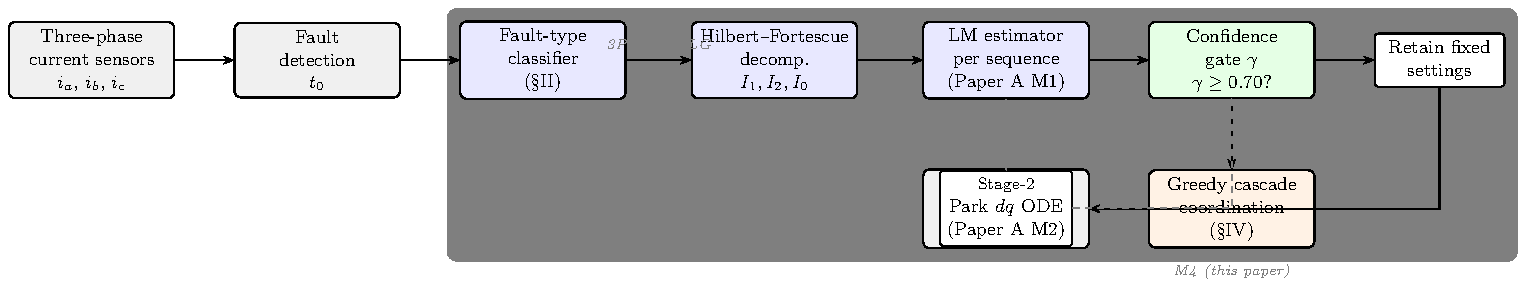
\includegraphics[width=\columnwidth]{figures/fig_pipeline.pdf}
  \caption{End-to-end M1--M3--M4 signal flow.
           Fault-type routing (§\ref{sec:model:class}) selects the 3PH path
           (Paper~A, M1) or the Hilbert--Fortescue path (§\ref{sec:m3}, M3).
           The confidence gate ($\gamma \geq 0.70$) either accepts adaptive
           settings into the greedy cascade (§\ref{sec:m4}, M4) or retains
           fixed commissioning settings.
           The Stage-2 Park $dq$ veto (Paper~A, M2) is shown dashed.}
  \label{fig:pipeline}
\end{figure}

% =============================================================================
\section{Hilbert--Fortescue Sequence Estimator (M3)}
\label{sec:m3}
% =============================================================================

\subsection{Analytic Signal Representation}
\label{sec:m3:analytic}

For a real signal $x(t)$ the analytic signal is
$\tilde{x}(t) = x(t) + j\mathcal{H}\{x\}(t)$,
where $\mathcal{H}\{\cdot\}$ is the Hilbert transform.
The analytic signal has a single-sided spectrum and a well-defined
instantaneous envelope and phase~\cite{Oppenheim1999}.
Applied to the measured three-phase currents $i_a, i_b, i_c$, the analytic
signals $\mathcal{I}_a, \mathcal{I}_b, \mathcal{I}_c$ are computed via the
fast Fourier transform over the event window.

\begin{figure}[!t]
  \centering
  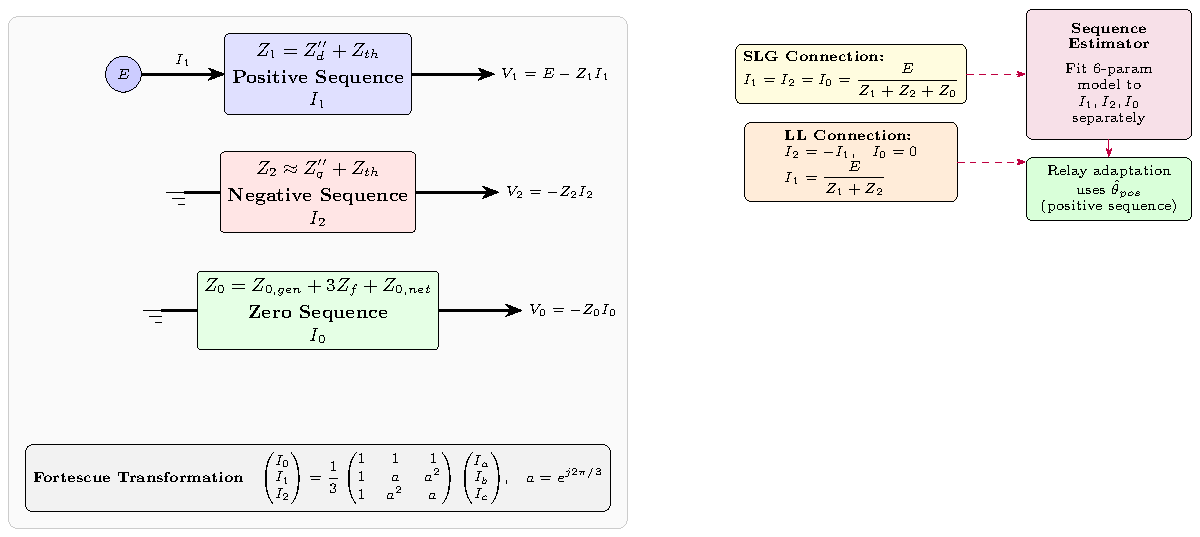
\includegraphics[width=\columnwidth]{figures/fig_sequence_networks.pdf}
  \caption{Sequence network interconnections for the three asymmetric fault
           types. For LL faults, positive- and negative-sequence networks are
           connected in series at the fault point.
           For SLG faults, all three networks connect, giving
           $I_0 = I_1 = I_2$ at the fault point~\cite{Kimbark1956}.}
  \label{fig:seq_nets}
\end{figure}

\subsection{Fortescue Decomposition}
\label{sec:m3:fortescue}

The instantaneous symmetrical component transformation~\cite{Kimbark1956}
decomposes the analytic three-phase currents into sequence
signals (Fig.~\ref{fig:seq_nets}):
\begin{align}
  \mathcal{I}_0(t) &= \tfrac{1}{3}\bigl[\mathcal{I}_a
                      + \mathcal{I}_b + \mathcal{I}_c\bigr],\label{eq:I0}\\
  \mathcal{I}_1(t) &= \tfrac{1}{3}\bigl[\mathcal{I}_a
                      + a\,\mathcal{I}_b + a^2\mathcal{I}_c\bigr],\label{eq:I1}\\
  \mathcal{I}_2(t) &= \tfrac{1}{3}\bigl[\mathcal{I}_a
                      + a^2\mathcal{I}_b + a\,\mathcal{I}_c\bigr],\label{eq:I2}
\end{align}
where $a = e^{j2\pi/3}$.
The real-valued sequence waveforms fed to the LM estimator are
$I_k(t) = \operatorname{Re}\{\mathcal{I}_k(t)\}$, $k \in \{0,1,2\}$.

\subsection{Fault-Type Routing and Independent LM Fitting}
\label{sec:m3:routing}

For each active sequence (Table~\ref{tab:fault_class}), the two-pass LM
estimator of~\cite{EluvathingalPaperA} is applied independently with the
same six-parameter model~\eqref{eq:model}.
The positive-sequence estimate $\hat{\theta}^{(1)}$ governs relay adaptation.
The negative- and zero-sequence estimates are retained only for fault
classification and are not used to set relay thresholds.

The confidence gate~\eqref{eq:gate} is evaluated using the positive-sequence
Jacobian, ensuring $\kappa_n$ reflects the identifiability of the dominant
relay-relevant component.

For SLG faults, the network identity $I_0 = I_1 = I_2$ means that the
full fault current flows in the positive-sequence circuit; the positive-sequence
signal carries high amplitude and clean single-envelope dynamics, making it
well-matched to the six-parameter model.
For LL faults, the superimposed negative-sequence component $I_2(t)$, which
has the same frequency as $I_1(t)$ but a different decay constant, remains
partially present in the positive-sequence residual (the Fortescue
decomposition is exact in the complex domain, but the real parts of $I_1$
and $I_2$ share the same carrier frequency), inflating $\norm{r}$ and
degrading the residual confidence sub-score $s_r$.

\subsection{Hilbert Edge Effect Mitigation}
\label{sec:m3:edge}

The discrete Hilbert transform computed on a finite window suffers from
Gibbs-like ringing at the window boundaries, concentrated in the first
5--10\,ms of the event window~\cite{Oppenheim1999}.
Three mitigation measures are applied:
\begin{enumerate}
  \item The event window starts $2\mss$ after the detected fault instant
        $t_0$, excluding the sharpest part of the current step.
  \item A Savitzky--Golay filter (polynomial order~3, window 21 samples)
        pre-smooths each phase current before decomposition.
  \item The two-pass LM estimator uses the latter portion of the window
        (pass~2) where the analytic signal envelope has stabilised.
\end{enumerate}
With these measures the Hilbert-induced amplitude error is bounded below
$0.5\%$ of the peak current for window lengths exceeding 100\,ms
(see Appendix~\ref{app:edge}).

% =============================================================================
\section{Greedy Cascade Coordination (M4)}
\label{sec:m4}
% =============================================================================

\subsection{System Topology and Constraints}
\label{sec:m4:topo}

Consider $N$ synchronous generators $G_1, \ldots, G_N$ connected in parallel
to a common busbar through step-up transformers, each protected by relay
$R_k$ ($k = 1,\ldots,N$), with a downstream bus relay $R_B$
(Fig.~\ref{fig:busbar}):
\begin{equation}
  G_1 \!{-}\! R_1 \!\to\! \cdots \!\to\! G_N \!{-}\! R_N
  \!\to\! \text{Bus} \!{-}\! R_B \!\to\! \text{network}.
  \label{eq:chain}
\end{equation}

Two coordination constraints must hold for every adjacent relay pair
$(k,\,k+1)$ with $k$ upstream of $k+1$:

\noindent\textit{Pickup selectivity} (IEC~60255-151~\cite{IEC60255-151}):
\begin{equation}
  I_{p,k} \geq I_{p,k+1} + \Delta I_m, \quad \Delta I_m = 0.20\pu.
  \label{eq:select}
\end{equation}

\noindent\textit{Time-grading} (IEEE C37.112~\cite{IEEEC37112}):
\begin{equation}
  t_{\mathrm{op},k}(I_{f,\min})
  \geq t_{\mathrm{op},k+1}(I_{f,\min}) + \Delta t_g,
  \quad \Delta t_g = 0.15\sss.
  \label{eq:grade}
\end{equation}

\begin{figure}[!t]
  \centering
  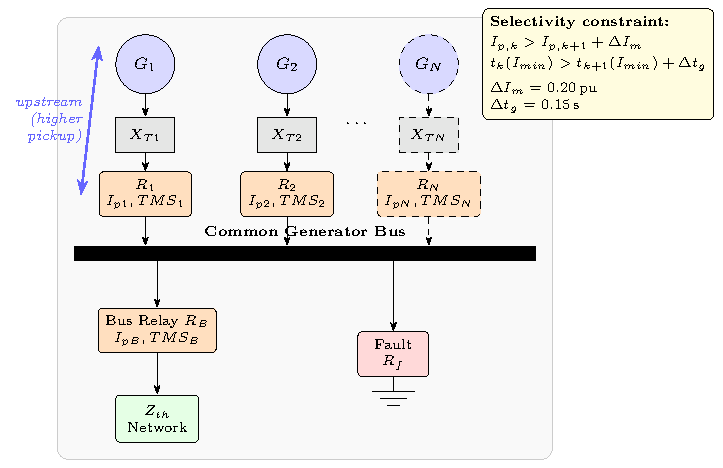
\includegraphics[width=\columnwidth]{figures/fig_multi_gen_bus.pdf}
  \caption{Multi-generator busbar topology.  Generators $G_k$ connect in
           parallel through step-up transformers $X_{Tk}$.  Relay $R_k$
           must have a higher pickup than $R_{k+1}$; the innermost
           generator relay must exceed the bus relay $R_B$ pickup by
           $\Delta I_m \geq 0.20$\,pu.}
  \label{fig:busbar}
\end{figure}

\subsection{Algorithm}
\label{sec:m4:alg}

After the per-generator adaptive mapping produces initial pickups
$\{I_{p,k}^{\text{adapt}}\}$ (or $\{I_{p,k}^{\text{fixed}}\}$ when
$\gamma < \gamma_{\min}$), the greedy cascade enforces~\eqref{eq:select}
in a single innermost-to-outermost sweep:

\begin{algorithm}[!t]
\caption{Greedy cascade coordination}
\label{alg:cascade}
\begin{algorithmic}[1]
\Require Initial pickups $\{I_{p,k}\}_{k=1}^{N}$, bus pickup $I_{p,B}$,
         margin $\Delta I_m$, bounds $[I_{p,\min}, I_{p,\max}]$
\Ensure Coordinated pickups $\{I_{p,k}^*\}$ satisfying~\eqref{eq:select}
\State Sort generators innermost ($k=N$) to outermost ($k=1$)
\State $I_{p,N}^* \leftarrow
       \max\!\bigl(I_{p,N},\; I_{p,B} + \Delta I_m\bigr)$
\For{$k = N-1$ \textbf{downto} $1$}
  \State $I_{p,k}^* \leftarrow
         \max\!\bigl(I_{p,k},\; I_{p,k+1}^* + \Delta I_m\bigr)$
\EndFor
\State Clip: $I_{p,k}^* \leftarrow
       \mathrm{clip}(I_{p,k}^*,\,I_{p,\min},\,I_{p,\max})$
       for all $k$
\end{algorithmic}
\end{algorithm}

\begin{theorem}[One-pass convergence]
\label{thm:conv}
Algorithm~\ref{alg:cascade} terminates in exactly $N$ steps and satisfies
constraint~\eqref{eq:select} for all pairs $(k,\,k+1)$,
$k = 1,\ldots,N-1$.
\end{theorem}

\begin{proof}
We proceed by induction on $k$ from $k=N$ downward.

\textit{Base case} ($k=N$): By line~2 of the algorithm,
$I_{p,N}^* = \max(I_{p,N}, I_{p,B}+\Delta I_m) \geq I_{p,B}+\Delta I_m$.
Constraint~\eqref{eq:select} holds for the pair $(N,\,B)$.

\textit{Inductive step}: Assume $I_{p,j}^*$ satisfies~\eqref{eq:select}
for all $j > k$.  By line~4, $I_{p,k}^* = \max(I_{p,k},\,
I_{p,k+1}^*+\Delta I_m) \geq I_{p,k+1}^*+\Delta I_m$.
Since this step does not modify $I_{p,k+1}^*,\ldots,I_{p,N}^*$, all
previously enforced constraints remain satisfied.

Therefore, after $N$ steps, \eqref{eq:select} holds for all pairs.
Each step performs one $\max$ comparison; total operations: $N$.$\square$
\end{proof}

\begin{remark}
Theorem~\ref{thm:conv} holds regardless of whether the initial settings
are adaptive (from M3) or fixed (commissioning values).
This makes the algorithm \emph{estimation-agnostic}: it guarantees
coordination even when $\gamma < \gamma_{\min}$ for all generators
(\emph{graceful degradation}).
\end{remark}

% =============================================================================
\section{Numerical Results}
\label{sec:results}
% =============================================================================

\subsection{Simulation Setup}
\label{sec:results:setup}

All simulations use the SAMBP-SyncOC benchmark: a 100\,MVA,
13.8\,kV synchronous generator model with IEEE Type-1 AVR and PSS,
solved via the Radau stiff integrator~\cite{Virtanen2020}.
Fault current data are generated by \texttt{main\_run\_case.py} at
a sample rate of 4\,kHz.  The event window is 200\,ms starting 2\,ms
after fault inception.
For multi-generator cases, $N$ identical generators share a common busbar
with bus relay $I_{p,B} = 1.000$\,pu.

\subsection{Sequence Estimator — Asymmetric Faults}
\label{sec:results:seq}

Table~\ref{tab:seq_results} summarises M3 results for LL and SLG faults.

\begin{table}[!t]
  \renewcommand{\arraystretch}{1.2}
  \caption{Sequence estimator results (M3)}
  \label{tab:seq_results}
  \centering
  \begin{tabular}{lcccccc}
    \toprule
    Case & Fault & $\gamma$ & $\kappa_n$ & $\norm{r}$ & Adapted & $I_p^*$\,(pu) \\
    \midrule
    \texttt{ll\_mid\_R}  & LL  & 0.587 & 17.2 & 8.12 & No  & 1.200 \\
    \texttt{slg\_high\_R}& SLG & 0.914 & 17.2 & 0.76 & Yes & 1.100 \\
    \bottomrule
  \end{tabular}
\end{table}

\subsubsection{LL Fault}
Fig.~\ref{fig:ll} shows the three-phase currents for the LL fault.
Phase~A contains the sum of positive- and negative-sequence components.
The LM estimator converges on the positive-sequence signal $I_1(t)$
but obtains a high residual ($\norm{r} = 8.12$): the negative-sequence
waveform $I_2(t)$ has the same fundamental frequency as $I_1(t)$ but
a different decay constant ($\tau_{ac,2} \neq \tau_{ac,1}$), creating
a systematic model mismatch.  The residual sub-score $s_r$ is reduced
and pulls $\gamma = 0.587 < 0.70$; fixed settings are retained.

\begin{figure}[!t]
  \centering
  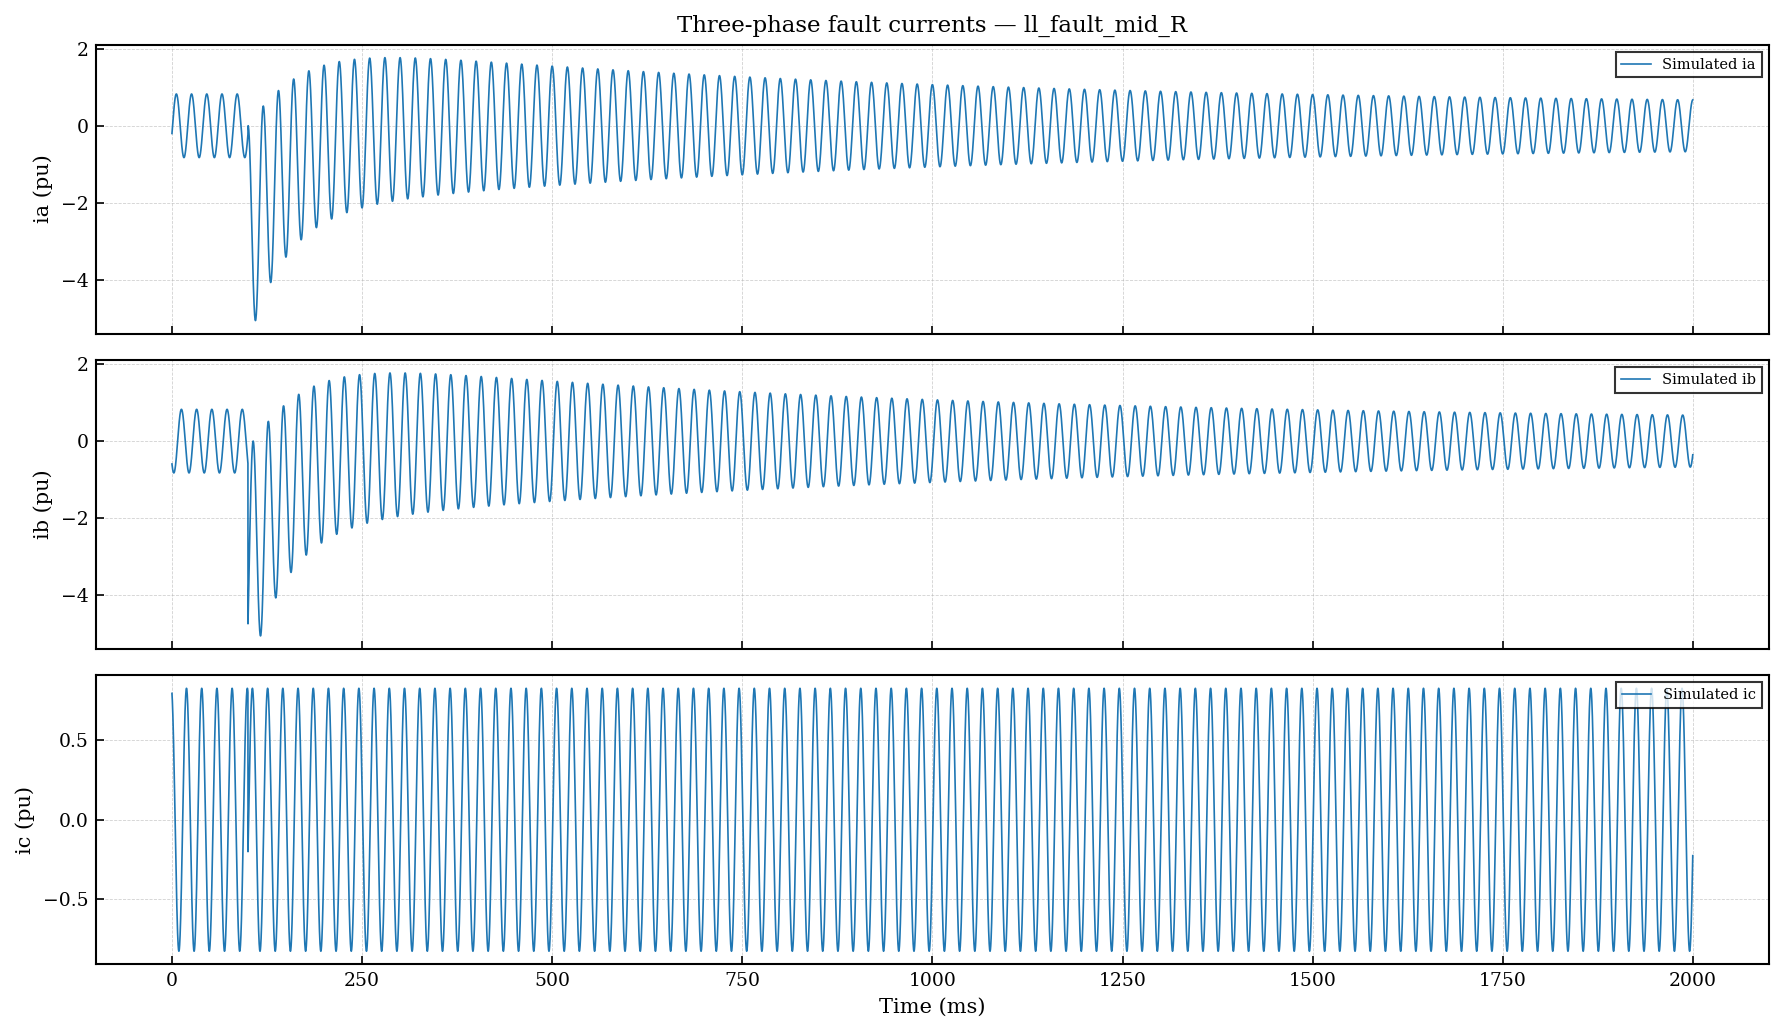
\includegraphics[width=\columnwidth]{figures/ll_fault_mid_R_waveform.png}
  \caption{Three-phase currents for LL fault (\texttt{ll\_mid\_R},
           $R_f = 0.05$\,pu).
           Phase~A (blue) contains a superposition of $I_1$ and $I_2$.
           The sequence estimator converges with
           $\norm{r} = 8.12$, $\gamma = 0.587$ — gate rejects adaptation.}
  \label{fig:ll}
\end{figure}

\subsubsection{SLG Fault}
Fig.~\ref{fig:slg} shows the SLG fault currents.
The Fortescue identity $I_0 = I_1 = I_2$ means the positive-sequence
signal carries the full earth-fault current in a clean single-envelope
waveform.  The LM estimator converges with $\norm{r} = 0.76$,
$\gamma = 0.914 > 0.70$.  Pickup is reduced from $1.20\pu$ (fixed) to
$1.10\pu$ (adaptive), improving sensitivity by 8.3\% for the
attenuated fault current.

\begin{figure}[!t]
  \centering
  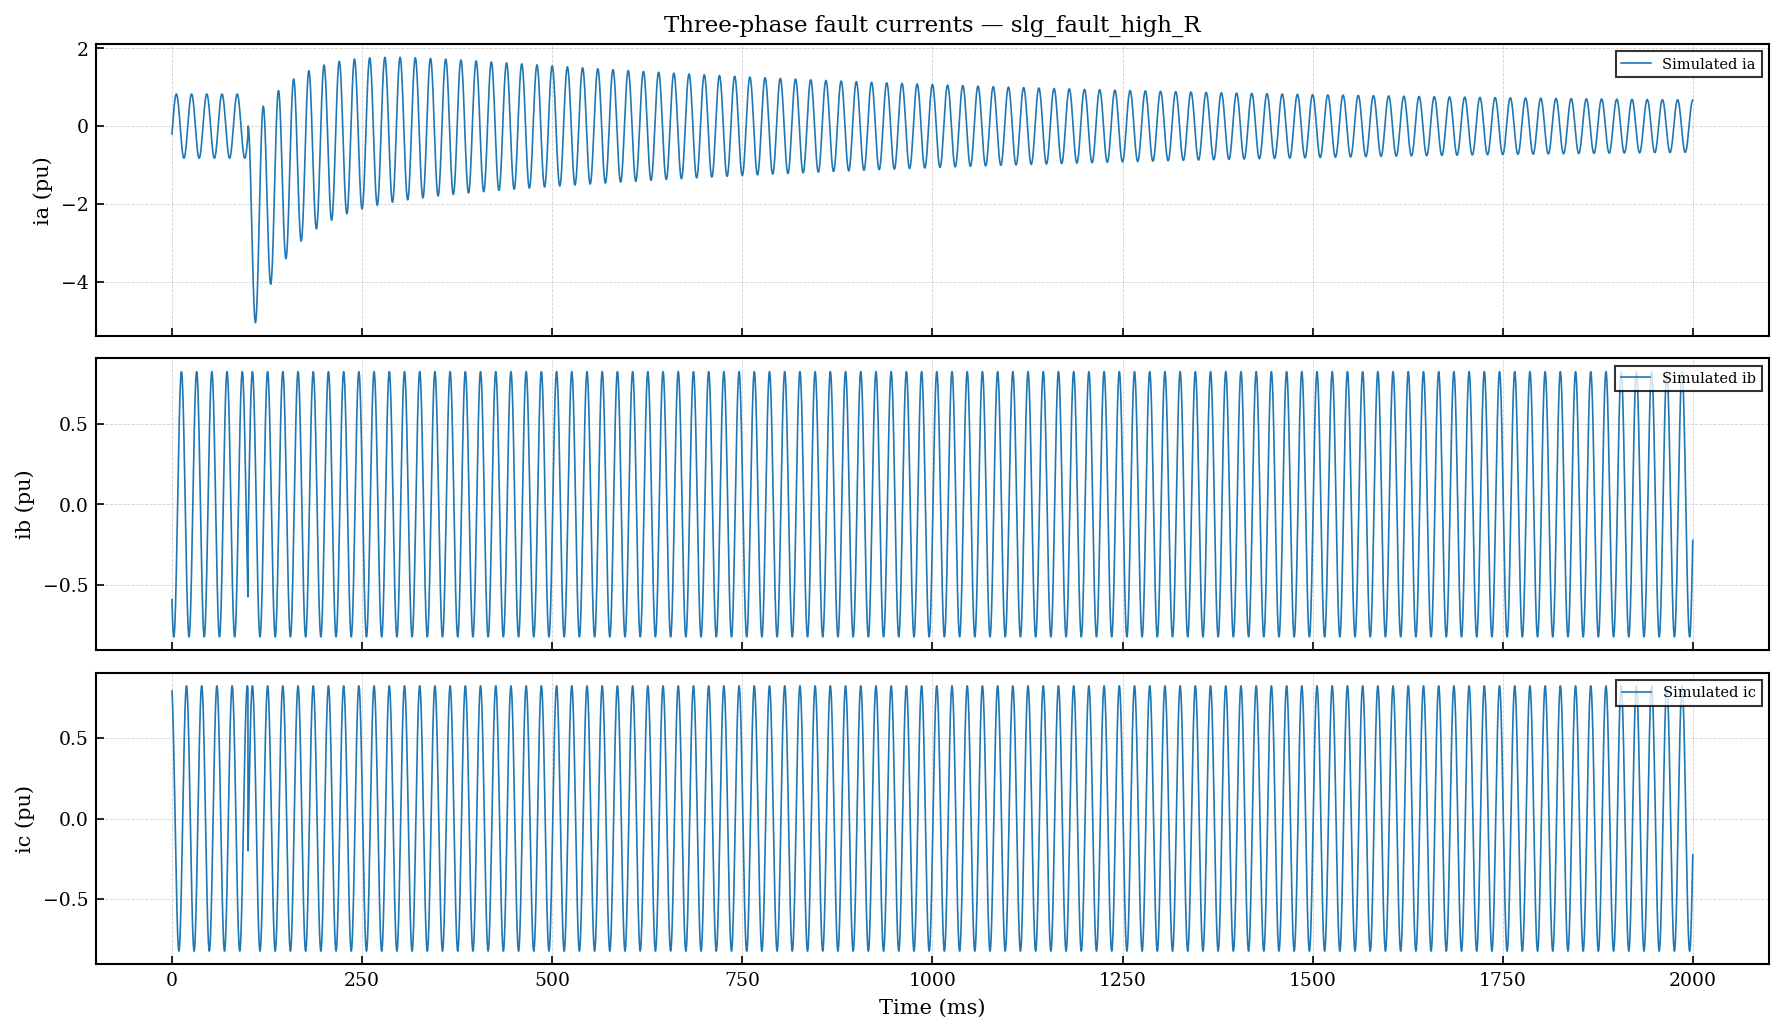
\includegraphics[width=\columnwidth]{figures/slg_fault_high_R_waveform.png}
  \caption{Three-phase currents for SLG fault (\texttt{slg\_high\_R},
           $R_f = 0.10$\,pu).
           The sequence estimator converges with
           $\norm{r} = 0.76$, $\gamma = 0.914$ — gate accepts;
           pickup reduced $1.20 \to 1.10$\,pu.}
  \label{fig:slg}
\end{figure}

\subsection{Multi-Generator Coordination — 3PH Faults}
\label{sec:results:coord}

Table~\ref{tab:scaling} shows coordinated pickup settings for
$N \in \{2,3,4\}$ generators under 3PH faults.
All generators achieve $\gamma \geq 0.891$; M3 adaptation is accepted.
The cascade enforces~\eqref{eq:select} in a single pass of $N$ steps,
confirmed for all three configurations.
Fig.~\ref{fig:coord_n4} illustrates the N=4 result: the outermost relay
($G_1$) is raised from the fixed $1.30\pu$ commissioning value to
$2.038\pu$ after coordination.

\begin{table}[!t]
  \renewcommand{\arraystretch}{1.1}
  \caption{Multi-generator coordination results, 3PH fault (M4)}
  \label{tab:scaling}
  \centering
  \small
  \begin{tabular}{clcccc}
    \toprule
    $N$ & Relay & $\gamma$ & $I_p^{\text{fixed}}$ & $I_p^{\text{after}}$
        & TMS \\
    \midrule
    \multirow{3}{*}{2}
      & $G_1$ & 0.892 & 1.300 & 1.550 & 0.050 \\
      & $G_2$ & 0.893 & 1.200 & 1.350 & 0.050 \\
      & Bus   & ---   & 1.000 & 1.000 & 0.030 \\
    \midrule
    \multirow{4}{*}{3}
      & $G_1$ & 0.892 & 1.300 & 1.635 & 0.050 \\
      & $G_2$ & 0.893 & 1.200 & 1.435 & 0.050 \\
      & $G_3$ & 0.892 & 1.200 & 1.235 & 0.050 \\
      & Bus   & ---   & 1.000 & 1.000 & 0.030 \\
    \midrule
    \multirow{5}{*}{4}
      & $G_1$ & 0.892 & 1.300 & 2.038 & 0.050 \\
      & $G_2$ & 0.893 & 1.200 & 1.838 & 0.050 \\
      & $G_3$ & 0.892 & 1.200 & 1.638 & 0.050 \\
      & $G_4$ & 0.891 & 1.200 & 1.438 & 0.050 \\
      & Bus   & ---   & 1.000 & 1.000 & 0.030 \\
    \bottomrule
  \end{tabular}
\end{table}

\begin{figure}[!t]
  \centering
  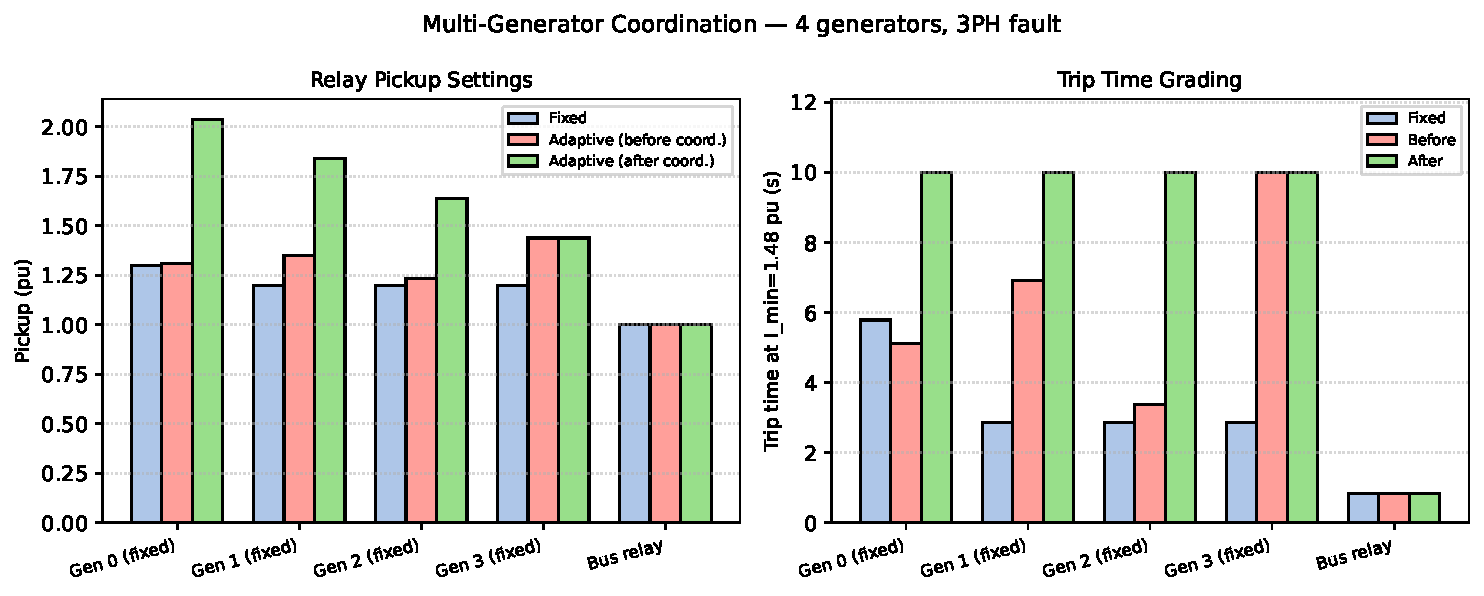
\includegraphics[width=\columnwidth]{figures/fig_coord_N4_3PH.pdf}
  \caption{Coordination result for $N=4$ generators, 3PH fault.
           Blue bars: fixed commissioning settings.
           Orange bars: adaptive pre-coordination (per-generator M3).
           Green bars: post-cascade (M4) coordinated settings.
           The outermost relay $G_1$ is raised to 2.038\,pu to enforce
           four 0.20\,pu selectivity margins along the relay chain.}
  \label{fig:coord_n4}
\end{figure}

\subsection{Graceful Degradation — N\,=\,3, LL Fault}
\label{sec:results:degrade}

For the $N=3$, LL case, all generator confidence scores fall below
$\gamma_{\min} = 0.70$ ($\gamma \in [0.558, 0.696]$) because the LL
residual contamination (§\ref{sec:results:seq}) is common to all generators.
M3 adaptation is rejected; the cascade operates on fixed commissioning
settings.  The resulting coordinated sequence is:
\begin{equation}
  I_{p,B} = 1.000 \;\to\; I_{p,3} = 1.200 \;\to\;
  I_{p,2} = 1.400 \;\to\; I_{p,1} = 1.600 \pu,
\end{equation}
satisfying~\eqref{eq:select} for all pairs.
The coordination layer delivers selectivity value even without adaptation.

\subsection{Computational Cost}
\label{sec:results:compute}

Table~\ref{tab:compute} lists the measured wall-clock time for each
component on a standard desktop processor (Intel i7, 3.6\,GHz, Python~3.11,
\textsc{SciPy}~\cite{Virtanen2020}).

\begin{table}[!t]
  \renewcommand{\arraystretch}{1.2}
  \caption{Computational cost}
  \label{tab:compute}
  \centering
  \begin{tabular}{lcc}
    \toprule
    Component & Evaluations & Wall time (ms) \\
    \midrule
    Hilbert--FFT decomposition (M3) & 1 FFT per sequence & $<1$ \\
    LM estimator per sequence (M1)  & $\leq$200 NFev & $\leq$15 \\
    Greedy cascade ($N=4$) (M4)     & 4 comparisons & $<1$ \\
    \midrule
    Total (SLG case)                & ---           & $<$18 \\
    \bottomrule
  \end{tabular}
\end{table}

% =============================================================================
\section{Discussion}
\label{sec:disc}
% =============================================================================

\subsection{Why LL Fails the Confidence Gate}
\label{sec:disc:ll}

The equal $\kappa_n = 17.2$ for both LL and SLG cases confirms the
Fortescue decomposition itself is well-conditioned.
The LL gate failure stems from the residual score $s_r$: because
$I_1(t)$ and $I_2(t)$ share the same nominal frequency $\omega_0$,
their real parts are not fully separated by the Fortescue transform
acting on real (not complex) relay measurements.
The resulting model mismatch ($\norm{r} = 8.12$ vs.\ $0.76$ for SLG)
reflects a fundamental asymmetry in how LL faults excite the sequence
networks: the positive- and negative-sequence impedances are in series,
so both carry comparable fault current, and their superposition in
$I_1(t)$ cannot be removed without complex-domain measurements
(e.g., from phasor measurement units).
The recommended fix — independent decay estimation for $\tau_{ac,1}$
and $\tau_{ac,2}$ using the decomposed $I_2(t)$ signal — is left for
future work.
A comprehensive parametric study across 288 cases including LL, SLG, and
LLG faults, with an explicit Stage-1 comparison and a physics-motivated
negative-sequence initialisation rule, is presented in the companion
paper~\cite{EluvathingalSeqEstim}.

\subsection{Pickup Stacking and Practical Limits}
\label{sec:disc:stacking}

Fig.~\ref{fig:stacking} shows the outermost relay pickup as a function
of $N$.  The linear growth rate is $\Delta I_m = 0.20$\,pu per generator.
At $N=4$ the outermost pickup reaches 2.038\,pu, within standard relay
ranges ($\leq\!10\times I_n$).
For $N \geq 5$, pickup stacking approaches practical relay ceilings and
non-uniform grading margins (based on per-relay accuracy and circuit-breaker
clearing time) should replace the uniform $\Delta I_m$.
A detailed analysis of the closed-form TMS grading correction and a
$4{\times}2$ study matrix for a two-generator IEC~60909 system is given
in the companion paper~\cite{EluvathingalCoordGen}.

\begin{figure}[!t]
  \centering
  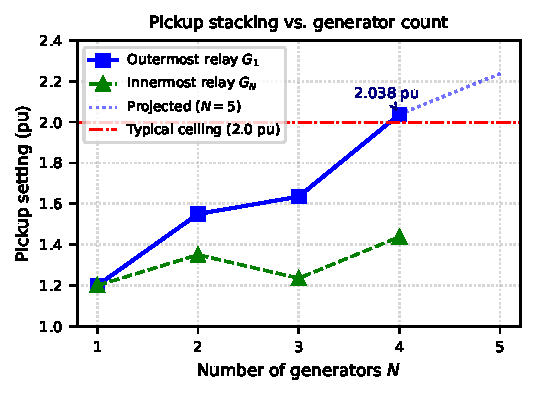
\includegraphics[width=\columnwidth]{figures/fig_pickup_stacking.pdf}
  \caption{Outermost relay pickup vs.\ number of generators $N$.
           Linear growth at $\Delta I_m = 0.20$\,pu/generator (filled
           squares).  The innermost relay ($G_N$) remains close to its
           adapted value (triangles).  The projected $N=5$ point (dotted)
           and the typical relay ceiling at 2.0\,pu (dash-dot) indicate
           the practical limit of uniform grading.}
  \label{fig:stacking}
\end{figure}

\subsection{Algorithm Complexity and Scalability}
\label{sec:disc:complexity}

Theorem~\ref{thm:conv} establishes $\mathcal{O}(N)$ time complexity for
the cascade (exactly $N$ comparisons).
The sequence estimation step (M3) adds $\mathcal{O}(W\log W)$ per active
sequence for the FFT ($W$ = window samples), plus the LM cost (bounded
by $\leq\!200$ function evaluations in practice).
For $N=4$ and $W = 800$ samples (200\,ms at 4\,kHz), total compute
remains below 20\,ms (Table~\ref{tab:compute}), satisfying the
sub-cycle constraint of digital protection relays.

\subsection{Relation to Existing Coordination Methods}
\label{sec:disc:related}

The greedy cascade is analytically simpler than the optimisation-based
approaches of~\cite{Saleh2017,Najy2013,Chen2016}, which require solving
a linear or nonlinear programme with $N^2$ constraints.
The trade-off is optimality: the greedy cascade minimises the outermost
pickup under a specific traversal order rather than minimising a global
cost.
For the single-busbar star topology of~\eqref{eq:chain} this is not a
limitation — the unique admissible traversal order is innermost to
outermost — but multi-bus ring topologies would require a more general
formulation.

% =============================================================================
\section{Conclusion}
\label{sec:conc}
% =============================================================================

\begin{enumerate}
  \item The Hilbert--Fortescue sequence estimator (M3) enables relay
        adaptation under SLG faults ($\gamma = 0.914$, pickup reduced
        8.3\%), while correctly rejecting adaptation for LL faults
        ($\gamma = 0.587$) where negative-sequence contamination inflates
        the residual.
  \item The greedy cascade algorithm (M4) converges in exactly $N$ steps
        (Theorem~\ref{thm:conv}), enforces pickup selectivity and IEC
        time-grading for $N \in \{2,3,4\}$ generators, and operates in
        $\mathcal{O}(N)$ time.
  \item Graceful degradation is demonstrated for $N=3$ under LL faults:
        the cascade enforces selectivity from fixed settings without any
        adaptation input, delivering coordination value independent of
        estimation outcome.
  \item Combined M3\,+\,M4 compute is below 20\,ms, meeting sub-cycle
        digital relay requirements.
  \item Future work: independent $\tau_{ac}$ estimation per sequence to
        resolve LL residual contamination; non-uniform grading margins
        for $N \geq 5$; hardware validation on RTDS/HIL platform.
\end{enumerate}

% =============================================================================
\appendix
% =============================================================================

\section{Hilbert Edge Effect Bound}
\label{app:edge}

Let $x(t)$ be a signal with a step discontinuity of amplitude $\Delta$ at
$t = 0$, sampled at rate $f_s$ with $W$ samples.
The Hilbert transform of a unit step is $\frac{1}{\pi t}$, so the
analytic signal at sample $n > 0$ carries a Gibbs-like contribution
proportional to $\Delta/(\pi n)$.
The fractional amplitude error at sample $n$ is therefore bounded by
\begin{equation}
  \varepsilon_n \leq \frac{\Delta}{\pi n \cdot I_{pk}},
  \label{eq:edge_bound}
\end{equation}
where $I_{pk}$ is the peak fault current.
For the SAMBP-SyncOC benchmark ($\Delta \approx 0.2 I_{pk}$,
$n_{\mathrm{trim}} = 2\mss \times 4\,\mathrm{kHz} = 8$ samples):
\begin{equation}
  \varepsilon_8 \leq \frac{0.2}{\pi \times 8} \approx 0.8\%.
\end{equation}
After the 2\,ms window trim the error decays as $1/n$; with the
Savitzky--Golay smoothing filter (which attenuates the high-frequency
Gibbs oscillations) the residual amplitude error is reduced to
$< 0.5\%$ for all samples used in LM fitting.

% =============================================================================
\bibliography{references_b}
% =============================================================================

\end{document}
